\documentclass[a4paper, 12pt]{article}%тип документа

%отступы
\usepackage[left=2cm,right=2cm,top=2cm,bottom=3cm,bindingoffset=0cm]{geometry}

%Русский язык
\usepackage[T2A]{fontenc} %кодировка
\usepackage[utf8]{inputenc} %кодировка исходного кода
\usepackage[english,russian]{babel} %локализация и переносы

%Вставка картинок
\usepackage{wrapfig}
\usepackage{graphicx}
\graphicspath{{pictures/}}
\DeclareGraphicsExtensions{.pdf,.png,.jpg}

%оглавление
\usepackage{titlesec}
\titlespacing{\chapter}{0pt}{-30pt}{12pt}
\titlespacing{\section}{\parindent}{5mm}{5mm}
\titlespacing{\subsection}{\parindent}{5mm}{5mm}
\usepackage{setspace}

%Графики
\usepackage{multirow}
\usepackage{pgfplots}
\pgfplotsset{compat=1.9}

%Математика
\usepackage{amsmath, amsfonts, amssymb, amsthm, mathtools}

%Стиль страницы
\usepackage{fancyhdr}
\pagestyle{fancy}

\begin{document}

\begin{titlepage}

\begin{center}
%\vspace*{1cm}
\large\textbf{Московский Физико-Технический Институт}\\
\large\textbf{(государственный университет)}
\vfill
\line(1,0){430}\\[1mm]
\huge\textbf{Работа 4.2.1}\\
\line(1,0){430}\\[1mm]
\vfill
\large Сибгатуллин Булат, ФРКТ\\
\end{center}

\end{titlepage}
\fancyhead[L] {Работа 4.2.1}
\noindent \textbf{Цель работы:} \\
\indent познакомиться с явлением интерференции в тонких пленках (полосы равной толщины) на примере колец Ньютона и с методикой интерференционных измерений кривизны стеклянной поверхности.\\
\noindent \textbf{В работе используются:} \\
\indent измерительный микроскоп с опак-иллюминатором; плоско-выпуклая линза; пластинка из черного стекла; ртутная лампа типа ДРШ; щель; линзы; призма прямого зрения; объектная шкала.

\section*{Экспериментальная установка}

На рис. 1. представлена схема наблюдения колец Ньютона. Найти радиус кривизны сферической поверхности такой линзы можно зная формулы для радиусов темных и светлых колец. Радиус темных колец:

\begin{equation}
r_m = \sqrt{m \lambda R}
\end{equation}

Радиус светлых колец:

\begin{equation}
r_m' = \sqrt{(2m - 1) m\lambda R/2}
\end{equation}

\begin{figure}[h!]
\centering
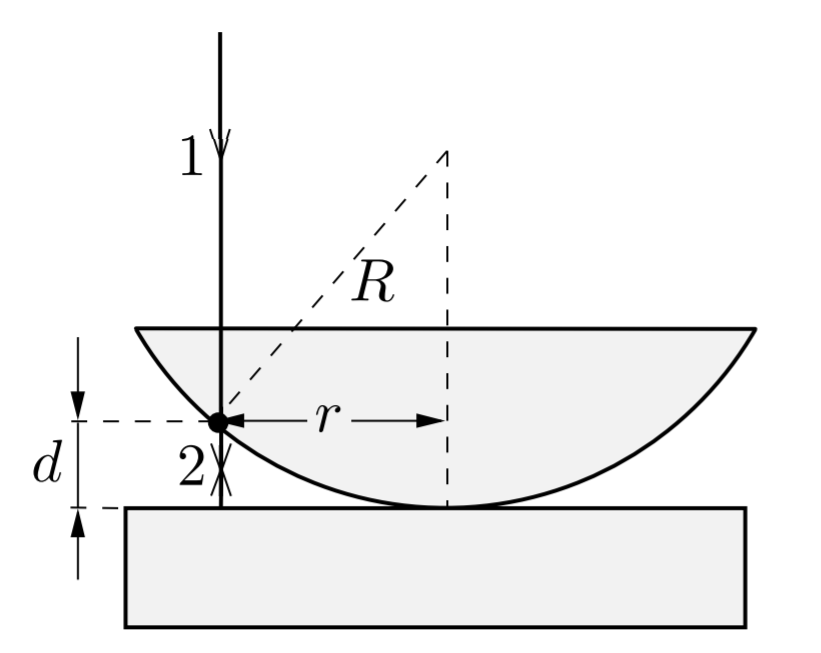
\includegraphics[scale=0.5]{images/scheme_0.png}
\caption{Схема наблюдения колец Ньютона}
\label{scheme_0}
\end{figure}

В нашей установке кольца Ньютона образуются при интерференции световых волн отраженных от границ тонкой воздушной прослойки заклюлченной между выпуклой поверхностью линзы и плоской стеклянной пластинкой.

Линии постоянной разности хода представляют собой концентрические кольца с центром в точке соприкосновения. Для протяженного источника линии равной толщины локализованы на поверхности линзы, если пластинка лежит на линзе, и вблизи поверхности линзы, если линза лежит на пластинке, как в нашем случае.

\vspace{0.5cm}

Схема экспериментальной установки представлена на рис. 1. Опыт выполняется с помощью измерительного микроскопа. На столике микроскопа помещается держатель с пластинкой черного стекла, на которой находится исследуемая линза.

\begin{figure}[h!]
\centering
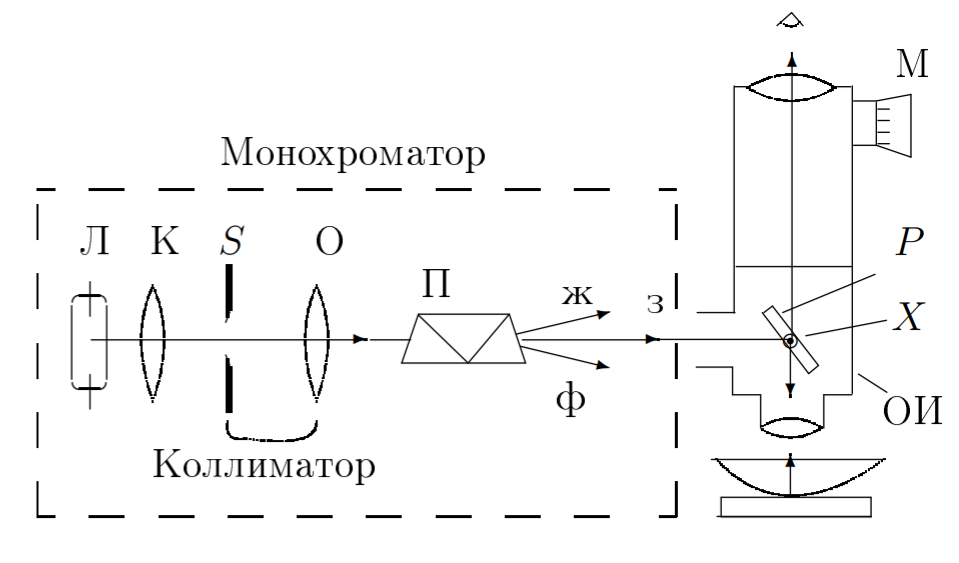
\includegraphics[scale=0.5]{images/scheme.png}
\caption{Схема установки для наблюдения колец Ньютона}
\label{scheme}
\end{figure}

Источником света служит ртутная лампа. Монохраматический свет получается в результате применения монохроматор, состоящий из конденсатора К, коллиматора (щель S и объектив O) и призмы прямого зрения П. Свет от монохроматора попадает на расположенный между объективом и окуляром микроскопа опак-иллюминатор (ОИ). Внутри опак-иллюминатора находится полупрозрачная стеклянная пластинка P, наколоненная под углом $45^{\circ}$ к оптической оси микроскопа. Свет частично отражается от этой пластинки, проходит через объектив и попадает на исследуемый объект.

Столик микроскопа может перемещаться в двух взаимно перпендикулярных направлениях с помощью винтов преперетоводителя. Отсчетный крест окулярной шкалы перемещается перпендикулярно оптической оси с помощью микроскопического винта М. Пластинка в опак-иллюминаторе может поворачиваться вокруг горизонтальной оси X, сам опак-иллюминатор  -- вокруг вертикальной оси.

\section*{Выполнение работы}

\end{document}